\documentclass[conference]{IEEEtran}
\IEEEoverridecommandlockouts
% The preceding line is only needed to identify funding in the first footnote. If that is unneeded, please comment it out.
\usepackage{cite}
\usepackage{amsmath,amssymb,amsfonts}
\usepackage{algorithmic}
\usepackage{graphicx}
\usepackage{textcomp}
\usepackage{xcolor}
\pagenumbering{arabic}
\def\BibTeX{{\rm B\kern-.05em{\sc i\kern-.025em b}\kern-.08em
    T\kern-.1667em\lower.7ex\hbox{E}\kern-.125emX}}
\begin{document}

\title{Using Neural Networks to generate test cases using BDD specifications}

\author{\IEEEauthorblockN{Nugawela, N. P. S. C.}
\IEEEauthorblockA{\textit{Department of Computer Science and Engineering} \\
\textit{University of Moratuwa}\\
Moratuwa, Sri Lanka \\
cnugawela@gmail.com}
}

\maketitle

\begin{abstract}
Testing is an integral part of software development. In recent times, ideologies such as TDD (Test Driven Development) and BDD (Behaviour Driven Development) have become popular. Here, we will be looking at BDD and how we can improve upon the current methods of implementing BDD and automating the process of impelmenting tests based on BDD. 
\end{abstract}

\begin{IEEEkeywords}
TDD (Test Driven Development), BDD (Behaviour Driven Development), GAN (Generative Adversarial Network), NLP (Natural Language Processing), POC (Proof Of Concept), SUT (System Under Test), GUI (Graphical User Interface)
\end{IEEEkeywords}

\section{Introduction}
The writing of tests for software projects has become very important in the modern era of software development. BDD has become a new trend wherein the test case is written in a user readable manner. The language used to specify the test cases is called Gherkin. Gherkin follows a simple format where a few select keywords are used to specify full user requirements.\cite{a1} The primary keywords are,
\begin{enumerate}
	\item Feature
	\item Example (or Scenario)
	\item Given, When, Then, And, But (steps)
	\item Background
	\item Scenario Outline (or Scenario Template)
	\item Examples
\end{enumerate}

There are some secondary keywords as well,

\begin{enumerate}
	\item """ (Doc Strings)
	\item | (Data Tables)
	\item @ (Tags)
	\item \# (Comments)
\end{enumerate}

Now we shall delve into the keywords in detail.
\subsection{Feature}
The purpose of the Feature keyword is to provide a high-level description of a software feature, and to group related scenarios.

The first primary keyword in a Gherkin document must always be Feature, followed by a : and a short text that describes the feature.

You can add free-form text underneath Feature to add more description.\cite{a1}

\subsection{Example}
This is a concrete example that illustrates a business rule. It consists of a list of steps. The keyword Scenario is a synonym of the keyword Example.You can have as many steps as you like, it is recommended that you keep the number at 3-5 per scenario. If they become longer than that, they lose their expressive power as specification and documentation.\newline
In addition to being a specification and documentation, a scenario is also a test. As a whole, your scenarios are an executable specification of the system.\newline
Examples follow this same pattern, \cite{a1}
\begin{itemize}
	\item Describe an initial context (Given steps)
	\item Describe an event (When steps)
	\item Describe an expected outcome (Then steps)
\end{itemize}

\subsection{Steps}
Each step starts with Given, When, Then, And, or But. Keywords are not taken into account when looking for a step definition. This means you cannot have a Given, When, Then, And or But step with the same text as another step.

\subsubsection{Given}
Given steps are used to describe the initial context of the system - the scene of the scenario. It is typically something that happened in the past. The purpose of Given steps is to put the system in a known state before the user (or external system) starts interacting with the system (in the When steps). Avoid talking about user interaction in Given’s. If you were creating use cases, Given’s would be your preconditions.

\subsubsection{When}
When steps are used to describe an event, or an action. This can be a person interacting with the system, or it can be an event triggered by another system.

It’s strongly recommended you only have a single When step per Scenario. If you feel compelled to add more, it’s usually a sign that you should split the scenario up into multiple scenarios.

\subsubsection{Then}
Then steps are used to describe an expected outcome, or result.

The step definition of a Then step should use an assertion to compare the actual outcome (what the system actually does) to the expected outcome (what the step says the system is supposed to do).

An observation should be on an observable output. That is, something that comes out of the system (report, user interface, message), and not something deeply buried inside it (like a database).

\subsubsection{And/But}
If you have several Given’s, When’s, or Thens, you could write:\cite{a1}

\begin{list}{*}{spacing}
	\item Example: Multiple Givens
	\item Given one thing
	\item Given another thing
	\item Given yet another thing
	\item When I open my eyes
	\item Then I should see something
	\item Then I shouldn't see something else
\end{list}

Or, we could make it read more fluidly by writing:
\begin{list}{*}{spacing}
	\item Example: Multiple Givens
	\item Given one thing
	\item And another thing
	\item And yet another thing
	\item When I open my eyes
	\item Then I should see something
	\item But I shouldn't see something else
\end{list}

\subsubsection{Background}
Occasionally we will need to repeat the same Given steps in all of the scenarios in a feature.

Since it is repeated in every scenario, this is an indication that those steps are not essential to describe the scenarios; they are incidental details. You can literally move such Given steps to the background, by grouping them under a Background section.

A Background allows you to add some context to the scenarios in the feature. It can contain one or more Given steps.

A Background is run before each scenario, but after any Before hooks. In your feature file, put the Background before the first Scenario.

You can only have one set of Background steps per feature. If you need different Background steps for different scenarios, you’ll need to split them into different feature files.\cite{a1}

\subsubsection{Scenario Outline}
The Scenario Outline keyword can be used to run the same Scenario multiple times, with different combinations of values.

The keyword Scenario Template is a synonym of the keyword Scenario Outline.
A Scenario Outline must contain an Examples (or Scenarios) section. Its steps are interpreted as a template which is never directly run. Instead, the Scenario Outline is run once for each row in the Examples section beneath it (not counting the first header row).\cite{a1}\newline

As you can see, the BDD test cases written in Gherkin have a high amount of structure that can be exploited. Currently, there are frameworks that support the generation and management of BDD test cases from Gherkin specifications. Some of the most popular frameworks used for BDD include,

\begin{itemize}
	\item JDave 
	\item Concordion 
	\item JBehave 
	\item Cucumber
	\item Serenity BDD
	\item SpecFlow   
\end{itemize}
These frameworks are used to map the requirements written in Gherkin style to the test code written in a programming language such as Java, .NET, etc. (Which is known as glue code\cite{a2}) So the programmers must still be ready to write the glue code for the Gherkin test cases. We seek to eliminate the necessity of this particular action.
In this paper we propose a novel method for generating test cases for software projects using recurrent neural networks, GANs, etc.

\section{Motivation}
Behaviour Driven Development is a practice that is being pushed within the agile practices. Many organizations are now adopting this practice in favour of having a set of comprehensive test documentation that supports multiple tiers within the organization.
\subsection{Making the test writing easy for the developer}
One of the major obstacles in the way of the adoption of BDD is the additional work a developer must put into writing the test cases. While there are frameworks such as Cucumber that support the writing of BDD testing, there is much to be desired. In the case of cucumber, we have to write the glue code by hand. It would be better if only we had to only write the Gherkin test case specifications.
\subsection{Allowing for greater automation}
Automation is very important for the current development environment as it is required to make deliveries on time to clients. Automating the generation of tests is a good path to take in the pursuit of optimizing the development process.
\subsection{Greater adoption of BDD}
BDD is a very good practice that has many benefits to offer the developers as well as Business Analysts, Managers, etc. So, it s very pleasing to see it being adopted in a greater capacity. So, as I pointed out before as well, the easy implementation of this practice will promote BDD greatly.


\section{Previous Work}
As I shall elaborate in the oncoming sections, there are many studies that are based on GANs. In those studies, it is usual to see the generation of images from random noise, \cite{b2} image generation using text descriptions, \cite{b5} and much more. Also there have been studies that consider the possibilities of employing GANs to cross domain fields.\cite{b3}\newline
There have not been any previous instances of generating BDD tests using text descriptions and GANs. So what I am suggesting is a novel venture, in terms of GANs.
There has been a code base aware test case generation in "Automatically Generating Tests from Natural Language Descriptions of Software Behavior" by Sunil Kamalakar.The problem description of this paper is as follows; "One weak point of BDD is the “glue code”—programmers are still required to produce
program “steps” that correspond to the basic actions described in the natural language scenarios. A number of tools have been developed to make the process of writing this glue code easier and streamlined, and to automatically map phrases in the scenarios onto such steps (typically using regular expressions). However, a manually-written bridge between the scenarios and the programmatic actions that correspond to them is still necessary.... The question we put forth is: Can we reduce the burden on programmers by utilizing information in the natural language, so that they don’t have to hand-write the glue code?"\cite{a2} 
The motivations mentioned in this paper are Increase in adoption of BDD, Ubiquitous communication and Reduction in effort, time and cost. These are very similar to our convictions as well.
The method proposed in the paper is as follows: "Our solution is to process the user stories written for BDD using state-of-the-art Natural Language Processing (NLP) techniques. Simultaneously, we scan the implementation/skeleton code of the project and capture every required property of the code, using reflection techniques. Once we have these two pieces, we employ a custom probabilistic matcher to map the BDD instructions onto code segments. Finally, based on the results of the probabilistic matcher, the code generator spits out code representing these mappings."\cite{a2}
The thesis by Sunil Kamalakar focuses on his work: \textit{Kirby}, a software tool written in Java, for auto-generating glue code from BDD scenarios. Kirby is capable of auto-generating code for projects implemented in Java. It outputs a specific code format in JUnit, which is a widely used unit testing framework for Java. The reason he has chosen Java is because, it is one of the most popular programming languages in use today, along with being a strictly object-oriented and typed-language.\cite{a2} Our approach differs from this approach as we seek to make the system support multiple programming languages and because we use neural networks.
Java has many frameworks and solutions supporting the adoption of BDD. Therefore, we focus on supporting other languages.

\section{Test Driven Development: Prelude To BDD}
In A Comparative Case Study on the Impact of
Test-Driven Development on Program Design and Test Coverage, it is mentioned that "Test-driven development (TDD) is a programming technique in which the tests are written prior to the source code. It is proposed that TDD is one of the most fundamental practices enabling the development of software in an agile and iterative manner. Both the literature and practice suggest that TDD practice yields several benefits. Essentially, it is claimed that TDD leads to an improved software design, which has a dramatic impact on the maintainability and further development of the system."\cite{b6} TDD in actuality is a development technique rather than a testing technique.\cite{b7} The tests are iteratively added throughout the implementation and when the tests pass, the code is refactored to improve its internal structure. This incremental cycle is repeated until all the functionality is implemented.\cite{b8} The idea of TDD was popularized by Beck\cite{b9} in the Extreme Programming (XP) method. Therefore, although TDD seems to have just recently emerged, it has existed for decades; an early reference to the use of TDD features in the NASA Project Mercury in the 1960s\cite{b10}. 
Both the literature and practice indicate that the use of
TDD yields several benefits. Among others, TDD leads to improved test coverage \cite{b8} and simplifies the design by producing loosely coupled and highly cohesive systems
\cite{b11}. TDD also enables the implementation scope to be more explicit. As a positive side effect, TDD may lead to enhanced job satisfaction and confidence \cite{b11}. Also, larger teams of developers can work on the same code base because of the more frequent integration\cite{b7}.  But, TDD has also been criticized for not
compensating the lack of up-front design and not being
very suitable for systems such as security software or
multithreaded applications, since it cannot mechanically
demonstrate that their goals have been met\cite{b12}. It is also
claimed that rapid changes may cause expensive
breakage in tests and that the lack of application or
testing skills may produce inadequate test coverage\cite{b13}. However, the scientific empirical evidence behind these
claims is currently scattered and disorganized, and thus it
is difficult to draw meaningful conclusions. Moreover,
studies addressing the impact of TDD on program design
are currently very rare\cite{b6}.
The work by Maria Siniaalto and Pekka Abrahamsson states that, The results partially contradict the current literature as the empirical evidence shows that TDD does not improve the program design as expected. In particular, TDD does
not necessarily produce highly cohesive systems when employed by non-professional developers. However, TDD appears to result in significantly better test coverage than the iterative test-last development. The findings are based on three software development projects, two of which used iterative test-last development and one utilized TDD\cite{b6}.\newline
Looking at another body of work by B. George and L. Williams, "..we find the definition of TDD as, before writing implementation code, the developer writes automated unit test cases for the new functionality they are about to implement. After writing test cases that generally will not even compile, the developers write implementation code to pass these test cases. The developer writes a few test cases, implements the code, writes a few test cases, implements the code, and so on. The work is kept within the developer’s intellectual control because
he or she is continuously making small design and implementation
decisions and increasing functionality at a relatively consistent rate. A new functionality is not considered properly implemented unless these new unit test cases and every other unit test cases ever written for the code base run properly.
"\cite{c1}
Maria Siniaalto et al. has compiled results from empirical studies conducted on TDD to evaluate the value of TDD as an engineering practice. In this study, they have looked at the studies of Bhat and Nagappan. They present the results of two
industrial case studies conducted at Microsoft. They
compared the impacts of TDD and non-TDD
development processes on quality and overall
development time. Their results show that the quality of
the code developed using TDD increased 2.6–4.2 times
when compared to non-TDD developed code.
Alternatively, the project managers estimated that TDD
increased the overall development time by 15–35 \%. The
block coverage was 79–88 \% at unit test level in projects
employing TDD. They also noticed that the tests serve as
auto documentation when the code was maintained or
used \cite{c2}. 
\section{Generative Adversarial Networks (GANs)}
\subsection{What is a GAN}

A GAN comprises of two neural network. One is used for model generation and the other is used for model validation. GANs are used in a variety of applications in the data science and machine learning domain. First introduced in the paper by I. J. Goodfellow, et at. titled "Generative Adversarial Nets" published in 2014. In it, they "propose a new framework for estimating generative models via an adversarial
process, in which we simultaneously train two models: a generative model G
that captures the data distribution, and a discriminative model D that estimates
the probability that a sample came from the training data rather than G." The adversarial modeling framework can be applied directly when the models are both
multilayer perceptrons. To learn the generator’s distribution $p_{g}$ over data x, they define a prior on input noise variables $p_{z}(z)$ then represent a mapping to data space as $G(z; \theta_{g})$, where G is a
differentiable function represented by a multilayer perceptron with parameters $θ_{g}$. We also define a
second multilayer perceptron $D(x; θ_{d})$ that outputs a single scalar. D(x) represents the probability
that x came from the data rather than $p_{g}$. We train D to maximize the probability of assigning the
correct label to both training examples and samples from G. We simultaneously train G to minimize
log(1 − D(G(z))). 
\cite{b1}\newline 

\subsection{Uses of GANs}

The scholarly work based on GANs include, using conditional generative adversarial nets for convolutional face generation wherein the authors, by varying the conditional information provided to an
extended GAN, use the resulting generative model
to generate faces with specific attributes from nothing but
random noise. 
An ideal training process for the above model would be
as follows: \begin{list}{*}{spacing}
	\item The generator outputs random RGB noise by default.
	\item The discriminator learns basic convolutional filters in
	order to distinguish between face images and random
	noise.
	\item The generator learns the correct bias (skin tone) and
	basic filters to confuse the discriminator.
	\item  The discriminator becomes more attuned to real facial
	features in order to distinguish between the simple
	“trick” images from the generator and real face images.
	Furthermore, the discriminator learns to use signals in
	the conditional data to look for particular triggers in
	the image.
\end{list} 

This process continues ad infinitum, until the discriminator
is maximally confused. Since the discriminator outputs
the probability that an input image was sampled from the
training data, we would expect a “maximally confused” discriminator
to consistently output a probability of 0.5 for
inputs both from the training data and from the generator.
\cite{b2} We can see that adversarial networks can be used to create useful cases of a target population and a model that would recognize the useful cases and filter them from a sample containing both useful and noise or unfit instances. Also, from this study we can see that even random noise can be used to generate useful instances.\newline
The authors T. Kim, M. Cha, H. Kim, J. Lee, and J. Kim have proposed a method based on generative adversarial networks that learns to discover relations between different domains
(DiscoGAN). Inter domain relationships are very obvious to people, unlike it is for machines. For example, we recognize the relationship between an English sentence and its translated sentence in French.It is fair to consider and contemplate whether machines can also discriminate and also see the inter-relationships among various domains. The authors have addressed this in the form of a conditional image generation problem. In other words, authors tried to find a mapping function from one domain to the other can be thought as generating an image in one domain
given another image in the other domain. The authors also note that this problem also brings an interesting challenge from a learning point of view as explicitly supervised data is seldom available and labeling can be labor intensive. Moreover, pairing images can become tricky if corresponding images are missing in one domain or there are multiple best candidates. So, the authors have resolved to automate the discovery of relations between two visual domains without any explicitly
paired data.\cite{b3} From this study we can deduce that it is possible to discover the relationships between two domains using GANs and thus generate a GAN that would use inputs from one domain to generate instances in another domain. Thus, it is justifiable to assume that it is feasible to generate test cases, which are formed conforming to the rules of a programming language such as C++, Java, Python, etc. from use cases specified in natural language.\newline

\section{Modern Software Development}
Modern software development involves much more than simple writing of code. Test driven development was the first step in creating code that was more reliable and consistent. With the recent popularity of agile methodology and push towards code quality, tests and test automation has become very important for development. Today, Test driven development has recently re-emerged as a critical enabling practice of the extreme programming software development methodology. L. Williams, E. M. Maximilien and M. Vouk ran a case study of this practice at IBM. In the process, a thorough suite of automated test cases was produced after UML design. In this case study, they found that the code developed using a test-driven development practice showed, during functional verification and regression tests, approximately 40\% fewer defects than a baseline prior product developed in a more traditional fashion. The productivity of the team was not impacted by the additional focus on producing automated test cases. This test suite aids in future enhancements and maintenance of this code. The case study and the results are discussed in detail.\cite{b4} From the study we can see that TDD can improve the quality of work and also can do so without impeding on the normal software development process. The current trend in software development are highly geared towards delivering quality software to clients, as quickly as possible. New methodologies such as Agile software development are being adopted in order to replace the old development methodologies such as waterfall. To accommodate this high quality and fast delivery process, it is imperative that the code is properly tested for the intended functionalities.\newline
Modern development definitely calls for TDD, but it is not sufficient. The test cases can be readable and understandable for the developer, but apart from the developer, people within the project such as business analysts and the client. So, the next innovation within the software development testing was to change the way that the tests are written and used.\newline
Now the move is towards the automation of tests and writing code that is much more comprehensible. Now, manual testing is discouraged and automated test writing is encouraged. The availability of free and open source tools for test automation such as Jenkins speaks volumes about the importance of test automation. Automated test cases allows for more efficiency and can immediately notify the developer in the case that the code is broken. In the case that there are manual tests instead of automated tests, the developer has to run the tests manually and see if code has been broken. This is a problem if there are too many tests to be run manually. The move now is also towards writing tests based on the client requirements. This way  the developers can make sure that the client requirements are aligned with the actual development process.\newline

\section{Behaviour Driven Development (BDD)}
\subsection{What is BDD?}
Behaviour Driven Development is a relatively new branch of development wherein the client requirements are used as the baseline for generating the test cases. This is a solution to the problems we have introduced during the last section. The test cases are based completely on the requirements provided by the client. So the development process will be completely aligned with the client requirements. This results in tests that test for the end-user use cases rather than much more abstract conditions.\newline
The business analysts can note down the client requirements in the following manner, highlighting their requirements so that it would be possible to discern the conditions required for user acceptance.
\begin{itemize}
	\item GIVEN: The client's initial state.
	\item WHEN: The change that takes place, it can be a change made by the client or some other event that takes place which is not controlled by the client.
	\item THEN: The expected behaviour when the change occurs.
\end{itemize}
We can translate such requirements directly into test cases. The methodology to be followed in such a scenario is as follows;
\begin{itemize}
	\item GIVEN: The starting condition. Initial conditions that we take are available at the start of the test.
	\item WHEN: The change that happens or is expected to happen. This is a disruptive event that will cause the event that will setup the expected response.
	\item THEN: The test scenario. The response that we are looking for after the disruption condition.
\end{itemize}

Following Fig. 1 is an example from the cucumber BDD test case.

\begin{figure}
	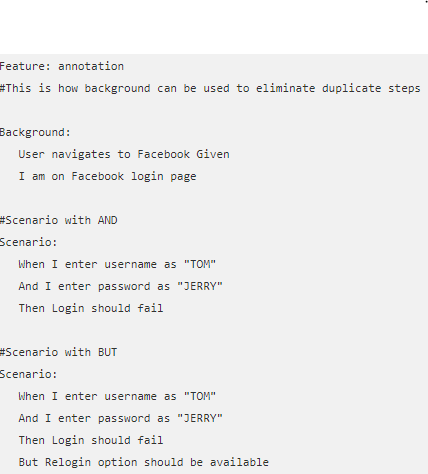
\includegraphics[width=\linewidth]{cucumber_figure.png}
	\caption{Example of Cucumber Test Execution}
	\label{fig1}
\end{figure}

\section{Generation of BDD compliant tests with Code Base Awareness}
\subsection{Justification}
Generation of test cases is akin to generating images using text. Han Zhang et al. have done a study wherein they synthesize high-quality images from text descriptions as samples generated by existing text-to-image approaches can roughly reflect the meaning of the given descriptions, but they fail to contain necessary details
and vivid object parts. The authors have had much success in generating images which fit the plain text descriptions of them, as specified.\cite{b5} Our case is similar in that we are using a user specified plain text to generate compilable and working test code. The success of the previous studies encourage us in that we can achieve our task of generating test cases directly from the plain text descriptions of the functionality.

\begin{figure}
	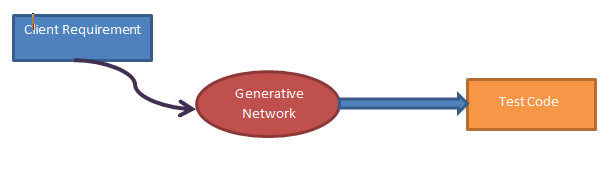
\includegraphics[width=\linewidth]{Generative_network.png}
	\caption{The functionality of the generative network}
	\label{fig2}
\end{figure}

\subsection{Initial Proposed Model}
This section describes the initial plan/proposal for the implementation of this system I came up with. Afterwards, it went through many refinements but some of the basics used here, remained.

\subsubsection{The Generative Network}
As displayed by the Fig. 2, the task of the generative network is to look at the client requirement of a functionality, here we introduce the constraint that it must follow a certain format. The format being the language we use when specifying a requirement when we write down a BDD test scenario. That is, it must follow the basic structure of,

\begin{itemize}
	\item Scenario
	\item GIVEN
	\item WHEN
	\item THEN
\end{itemize}

\begin{figure}
	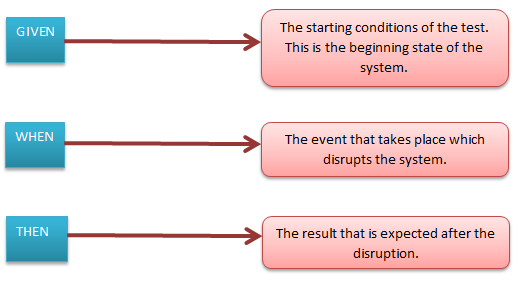
\includegraphics[width=\linewidth]{Given_when_then.png}
	\caption{BDD Test case structuring}
	\label{fig3}
\end{figure}

based on the descriptions, the generative network will be able to infer class names and their members, methods and their signatures.

\subsubsection{Validation Network}
The validation is done with two validation networks. Here, we have a network that checks the code compilation validity and another network that checks the validity of the generated code against the initial customer requirement.

\begin{figure}
	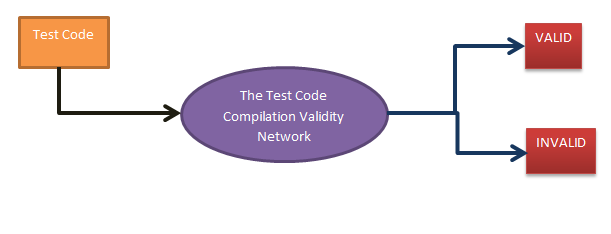
\includegraphics[width=\linewidth]{Compilation_validity.png}
	\caption{Compilation validity checking network}
	\label{fig4}
\end{figure}

\begin{figure}
	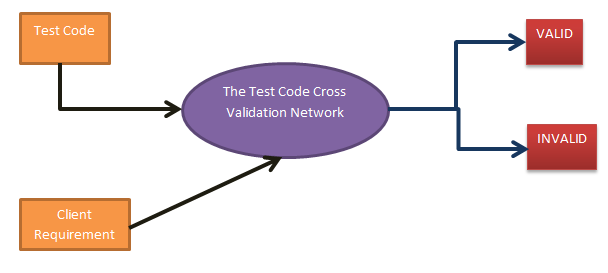
\includegraphics[width=\linewidth]{Cross_validation.png}
	\caption{Cross validation checking network}
	\label{fig5}
\end{figure}

The validation networks, as specified here, are suggestions based on the functionality and can be unified if necessary.

\subsection{The Generative Network}
The generative network is responsible for the generation of the BDD style test cases based on the client requirements given. This network should have a natural language processing capability that can reliably process the client requirement. This module must be capable of going through the requirement and deciding the necessary classes, methods and their signatures. Also, since the test is specified in the Given-When-Then style, this module must be capable of determining the control flow of the test, quite easily as well.\newline
The module that succeeds the Natural Language Processing (NLP) module is the module that can generate the test case based on the abstract output of the previous module. Note that we explicitly used the term \textit{abstract} to describe the output of the NLP module. This is due to the fact that, we would like the output to be language agnostic so that we can use the output to generate code of any language. As a result, the code generation module can be programmed to generate code in any language. As a result, we can make the code generation module for generating code for Java, C++, Python, JavaScript, etc. and thus we can have multiple code generation modules rather than a single code generation module. Such a setup is useful if we have code bases in multiple programming languages, as it is sometimes practiced in organizations to have code bases in different languages but the same functionality.

\begin{figure}
	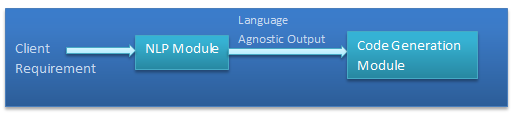
\includegraphics[width=\linewidth]{Gen_net_modules.png}
	\caption{Generative network modules}
	\label{fig6}
\end{figure} 

\begin{figure}
	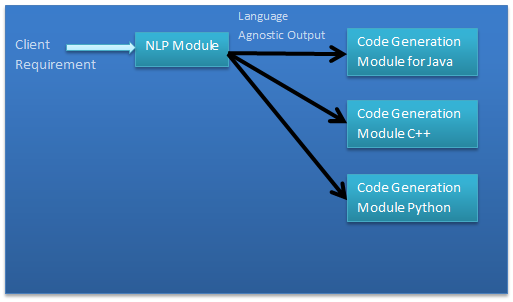
\includegraphics[width=\linewidth]{Gen_net_modules_multiple.png}
	\caption{Generative network modules with support for multiple languages}
	\label{fig7}
\end{figure} 

\subsection{The Discriminative Network}

The discriminative network will decide whether the output of the code generation module is valid. This can be done in two ways.

\begin{enumerate}
	\item\textit{Code consistency checking} : Checking whether the generated code is consistent with the rules of the target programming language.
	\item\textit{Consistency with client requirement} : This is checking whether the generated code is consistent with the client requirement. It involves NLP. 	
\end{enumerate}

Both of these are not programming language agnostic as the output of the code generation module is programming language specific. So if we need to support multiple languages, we will need multiple verification modules. Also it is advisable to have two modules to perform the aforementioned two tasks, with a module for each checking case. The complete validation module, thus achieved, is presented in the Fig. 9.\newline
The results from the verification modules are fed back to the generative modules to improve upon their generative process, so that as time goes on, the generative procedure will improve tot the point that the verification module will not distinguish between the actual valid cases and the generated cases that are fed to it.\newline
The code only verification module of the validation module set acts as the basic sanity test the generative network has to pass. Actually, we can first train with the code only verification module as the sole component of the discriminative network and then after it is satisfied, move onto the code and client requirement cross validation module.

\begin{figure}
	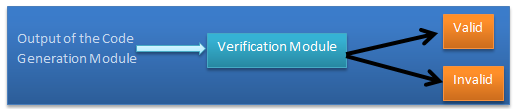
\includegraphics[width=\linewidth]{Validation_module.png}
	\caption{The basic validation module}
	\label{fig8}
\end{figure} 

\begin{figure}
	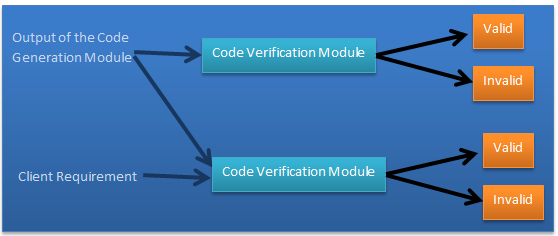
\includegraphics[width=\linewidth]{Complete_verification_module.png}
	\caption{The complete validation module set}
	\label{fig9}
\end{figure}

\subsection{Combined system} 
The combined system, comprising of the generative network and the adversarial network,  will take as inputs, client requirement specifications (Written in plain text, adhering to the BDD principles.) and generate compilable/interpretable test cases, in a target programming language or languages. The adversarial network attempts to reject these generated test cases. As the GAN evolves with time, the adversarial network becomes more and more confused between the generated test cases and true manually written test cases, ending when it cannot distinguish between manually written test cases and generated test cases.

\subsection{Training}
For the training of the GAN, we use client requirements alongside with proper test cases written to represent them in our desired language. Here, a single language is specified because we would have to train separately to support for multiple languages. Here we would only consider the case where a single programming language is present.\newline
Concerning the classes and methods that are available to generate the tests, we can train the neural networks on the available classes and their structure. Or we can allow the network to generate the class stubs based on the client requirements. Only the discriminative network needs to be attuned to the available code base as it can tune the generative network to use the correct classes, members and methods. But it is wise to tune the generative network in advance in order to minimize training times. Apart from the developer created classes, the GAN must also learn the basic data types of the language such as int, float, etc. and language provided data structures such as vectors, arrays, maps, etc. This is further more complicated when the developers use $3^{rd}$ party libraries, as we have to train for their specifics as well. So as to simplify matters, the first iteration can cover a subset of tests that are lower in complexity. The NLP module is used to extract the relevant tags that are useful to us from the plain text client requirement specification. It can be a neural network or otherwise. It is also notable that it is not imperative to have the NLP module as we can make the code generation module absorb that complexity as well. But, we can benefit hugely from having a separate NLP module for tag extraction as it is reusable, so therefore, it is worthwhile to have the NLP module.\newline
The discriminative model testing plan is done via feeding the valid test cases as input to the verification module (That discriminates between valid and invalid test case as far as programming language consistency is concerned. i.e. the code only verification module) as valid inputs during feedback and feeding invalid test cases as invalid inputs. (during feedback) This will train the discriminative network to distinguish between the valid and invalid. We also have to train the client requirement cross validation module in a similar fashion as well. Here, we have 3 combinations.

\begin{enumerate}
	\item \textit{The test case is consistent with the client requirement} : Valid state is fed back to the network.
	\item  \textit{The test case is not consistent with the client requirement} : Invalid state is fed back to the network.
	\item  \textit{The client requirement is inconsistent/incoherent} : Invalid state is fed back to the network.
\end{enumerate}  

Here, we consider that if the test case itself is inconsistent with the programming language falls under the $2^{nd}$ scenario. The $3^{rd}$ case deals with the scenario that the specified client requirement is wrongly stated. This can be due to meaningless client requirements, client requirements not being specified according to the guidelines, badly specified requirements, etc.

\begin{figure}
	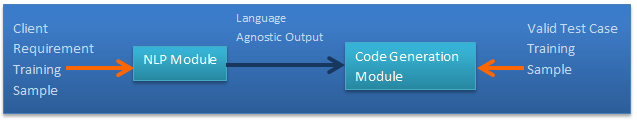
\includegraphics[width=\linewidth]{Generative_model_training.png}
	\caption{Generative model training plan}
	\label{fig10}
\end{figure} 

\begin{figure}
	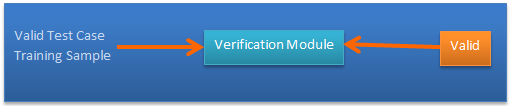
\includegraphics[width=\linewidth]{Discriminative_model_training.png}
	\caption{Discriminative model valid instance training plan}
	\label{fig11}
\end{figure} 

\begin{figure}
	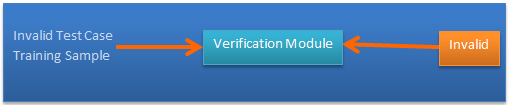
\includegraphics[width=\linewidth]{Validation_module_negative.png}
	\caption{Discriminative model invalid instance training plan}
	\label{fig12}
\end{figure} 

\subsection{Suggestions on implementation for the initial suggestion}
The first iteration of the GAN can be formed for simple cases such as basic arithmetic operations, simple algorithmic tasks and the like to train a basic GAN as a Proof Of Concept (POC) exercise. We also suggest adhering to structure of GIVEN, WHEN and THEN structure of test scenario writing within the client requirement specifications. Also, it will be practical to have only one target programming language for this first iteration.
Client requirement processing can be extended to include spell and grammar correction to try to form meaningful requirement specifications. Also we can expand the code base of the GAN's neural network so it can form much more complex test cases.

\section{Refined Modular Design}
The new design of the system is discussed in this section. We intend to support multiple programming languages in this approach. The model has been expanded and elaborated upon. Now, there are 5 major modules in the system. They are:

\begin{figure}
	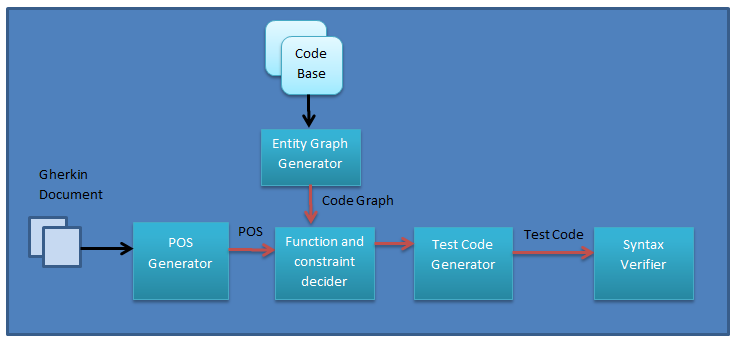
\includegraphics[width=\linewidth]{Complete_high_level_modules.png}
	\caption{Complete high-level model}
	\label{fig13}
\end{figure}

\begin{enumerate}
	\item \textbf{The POS/tags generator:}
	Breaks down the Gherkin test case to useful text tags. This is a NLP module. Does not depend on the programming language selection.
	\item \textbf{Entity Graph generator:}
	Scans the whole code base and breaks them down into a useful format that is understood by our system. (Actually, by the third module)
	\item \textbf{Function and constraint decider:}
	Looks at the tags and the code representation given to the module and decides the text-to-code mappings. This has NLP elements as well. Depends on the programming language selection.
	\item \textbf{Test Code generator:}
	Based on the selections and decisions, create the test case. Depends on the programming language selection. This is the generative section of the GAN.
	\item \textbf{Syntax verifier:}
	
\end{enumerate}

Let's examine the modules in detail in the next section.

\subsection{The POS/tags generator}
This module is capable of reading Gherkin files. It will process a single file at a time. The target of this module will be to extract the necessary tags from the file. Here, we will be considering the types of data that is contained within each of the cases in BDD. Let us examine the types of data that can be extracted from each of the Gherkin keywords.

\begin{itemize}
	\item \textbf{Feature:}
	Feature is the first keyword that we encounter when processing BDD specs. It is the topic under which the test cases are organized. Following the feature, there are lines describing the overall feature, which is usually used as comments. but we can use it for the deduction of functionality, but we must give it less emphasis as it is used as comments in most cases. It may be possible to discover functional and member bindings within the class through the feature descriptions.
	\item \textbf{Example/Scenario:}  
	This is the specification of a scenario, i.e. a BDD test case. From this section we can extract the name for the test case. Following this section are all of the step definitions, which make up the test case scenario. These will be the major source for the extraction of relationships.
	\item \textbf{Steps:}
	These contain the keywords, Given, When, Then, And, But. Given provides the initial setup conditions. The initial step should describe how the initial setup is done with enough clarity to unambiguously decide the classes and methods to call. We have to identify and pass the possible class and method and variable names and their relationship indicating words forward through the system. When represents a disruption within the system, hence it would be a specific input, either it is a certain signal or an object that is passed to the SUT. When is concerned about the output of the SUT. So to facilitate the recognition of these entities, we should pass the text values that would allow for the successful identification of the values for these entities and the ways in which we can capture these values.
	\item \textbf{Background:}
	Background is similar to a given statement that spans throughout multiple test cases. So we can treat it similar to the way we would treat a "Given" statement.
	\item \textbf{Scenario Outline:}
	The Scenario Outline keyword can be used to run the same Scenario multiple times, with different combinations of values. \ref{fig13} demonstrates an instance where a scenario outline is used \cite{a1}. Here, we can see the test case being parameterized and given multiple values for the input, signal and output values. Our system should be able to identify the parameters and the values associated with them, and pass them forward.
	\item \textbf{Doc Strings:}
	The doc string is passed as the last argument of a step definition when it is specified. We have to treat the string as an immutable value and pass it forward through the system.
	\begin{figure}
		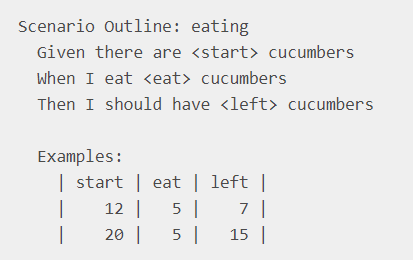
\includegraphics[width=\linewidth]{Scenario_outline.png}
		\caption{An example of a scenario outline}
		\label{fig13}
	\end{figure}
\end{itemize}

The NLP processing of the Gherkin test cases must preserve the relationships between the entities when generating the output. Since the test case is broken into sections by the Gherkin keywords, we can first split the processing along this separation first. Then given such a statement, we have to break it to possible class, method and value attributes and tag them as such. Then the "Function and Constraint Decider" can attempt to match them  with the existing code base.
 \subsection{Language Decider}
The language decider looks at the code base and decides what the target language is for the test case generation. Then, it loads the corresponding language modules in the Entity Graph Generator and Test Case Generator modules.
 
\subsection{Entity Graph Generator}
This module is responsible for parsing the available code base and generating a relationship graph which includes all of the available classes, their methods, inheritance and association relationships. This is created for the use in the "Function and constraint decider". The complexity here is that we are targeting multiple languages. There are two approaches we can take.

\begin{itemize}
	\item Implementing a system to identify the code from several languages.
	In this approach, we have to code the module to understand all of the target language's linguistics and thus generate the relationship graph. The module need not be able to distinguish between the languages unless there is a strict need to do so. (Such as, if the code base contains implementations of the same system in multiple languages.) It takes a considerable amount of coding on our part to handle all of the requisite languages.
	\item Using a neural network based solution. We can have multiple networks for each of the languages. But, in this solution, we need to have enough test scenarios of code and their graph representations to train the network.
\end{itemize}

\subsection{Function and constraint decider}
This section takes in the outputs of the previous two sections and tries to map the test case's entities to the entities from the code base graph. A NLP based difference checking between the entities in the test case and the entities in the code base graph. The major problem faced here is how to search for a specific keyword within the entity relationship graph. The solution we shall suggest is a tiered search. The search will start from the module to which the test case belongs. Then it will move to search the other directories.
We need a similarity measure to decide if there is a match between the BDD entity and the source code entities. Such measures can be,

\begin{enumerate}
	\item \textbf{A string matcher:} A simple string matcher that matches the class, method names using basic string operations.
	\item \textbf{An NLP matcher:} A matcher that considers the similarity between the two strings by considering the real life language meanings.
	\item \textbf{A context based matcher:} A matcher that attempts to match the entities based on descriptions and other relationships contained in the test case.
\end{enumerate}
 We opt to choose the last option as it provides the best opportunities for matching. The overall cost of operation for the module will be higher in this case than others and will take longer to find the final result.\newline
 Also, we will have to verify the decisions we have come up with the users. This is essential to avoid false positives in our search process. Therefore, this module must implement a GUI interface for the clients to interact with the program. The GUI should query the user when there are multiple possible matches or when there appears to be no matching entities to use. The user must be capable of manually resolving these problems. But, our goal is, given that the user, (or rather, the programmer who wrote the code) has followed standard accepted design principles, there will be no need for such disambiguation.\newline
 Once we have decide on the entities required to generate the test case, we shall pass the details learned to the test case generator.
 

\section{Conclusions}
In the modern software development ecosystem it is imperative to deliver high quality software products to the clients efficiently. TDD and lately, BDD have helped tremendously to achieve these goals. The problem of generating test cases for user specified scenarios with awareness of the existing code base is a novel and a promising one which can help organizations and individuals to develop better code. Here we have outlined a proposal for generating BDD test cases automatically. We do not have to specify a target language for the test cases, as we can allow for the system to discover that on its own.

\begin{thebibliography}{00}
\bibitem{a1} "Gherkin Reference", https://docs.cucumber.io/gherkin/reference/, 31st October 2018
\bibitem{a2} Sunil Kamalakar, "Automatically Generating Tests from Natural Language Descriptions of Software Behavior" \textit{Thesis submitted to the Faculty of the
	Virginia Polytechnic Institute and State University
}
\bibitem{b6}Siniaalto, Maria \& Abrahamsson, Pekka. "A Comparative Case Study on the Impact of Test-Driven Development on Program Design and Test Coverage". ESEM.2007., 2007, pp. 275 - 284.
\bibitem{b7}Beck, K., "Test-Driven Development By Example", AddisonWesley,
Boston, MA, USA, 2003.
\bibitem{b8}Astels, D., "Test-Driven Development: A Practical Guide",
Prentice Hall, Upper Saddle River, New Jersey, USA, 2003.
\bibitem{b9}Beck, K., Extreme Programming Explained, Second Edition:Embrace Change, Addison-Wesley, Boston, MA, USA, 2004.
\bibitem{b10}G. Larman and V.R. Basili, "Iterative and Incremental Development: A Brief History", IEEE Computer 36(6), IEEE Computer Soc., Los Alamitos, CA, USA, 2003, pp. 47-56.
\bibitem{b11} K. Beck, "Aim, fire", IEEE Software 18(5), IEEE Computer
Soc., Los Alamitos, CA, USA, 2001, pp. 87-89.
\bibitem{b1} I. J. Goodfellow, J. Pouget-Abadie, M. Mirza, B. Xu, D. Warde-Farley, S. Ozair, A. C.
Courville, and Y. Bengio, "Generative adversarial
nets." In Proceedings of NIPS, pages 2672–
2680, 2014
\bibitem{b12}Stephens, M. and D. Rosenberg, "Extreme Programming
Refactored: The Case Against XP", Apress, Berkeley, CA, USA,
2003.
\bibitem{b13}Boehm, B. and R. Turner, Balancing Agility and Discipline
- A Guide for the Perplexed, Addison-Wesley, Boston, MA,
USA, 2004.
\bibitem{c1}B. George, L. Williams, "An Initial Investigation of Test Driven Development in Industry", Proc. ACM Symp. Applied Computing, 2003.
\bibitem{c2}Bhat, T. and Nagappan, N. Evaluating the efficacy of testdriven
development: industrial case studies. In ISESE '06, Rio
de Janeiro, Brazil, 2006.
\bibitem{b2} J. Gauthier. "Conditional generative adversarial nets for
convolutional face generation." \textit{Class Project for Stanford
CS231N: Convolutional Neural Networks for Visual Recognition,
Winter semester,} 2014(5):2, 2014.
\bibitem{b3}T. Kim, M. Cha, H. Kim, J. Lee, and J. Kim. "Learning to discover cross-domain relations with generative
adversarial networks." International Conference on Machine Learning, 2017.
\bibitem{b4} L. Williams, E. M. Maximilien and M. Vouk, "Test-driven development as a defect-reduction practice", 14th International Symposium on Software Reliability Engineering, 2003. ISSRE 2003., 2003, pp. 34-45.
doi: 10.1109/ISSRE.2003.1251029
\bibitem{b5} H. Zhang, T. Xu, H. Li, S. Zhang, X. Huang, X. Wang, and D. Metaxas,
"Stackgan: Text to photo-realistic image synthesis with stacked generative
adversarial networks," arXiv preprint arXiv:1612.03242, 2016.
\end{thebibliography}
\vspace{12pt}

\end{document}
